\chapter{Some basic relationships of fluid mechanics and thermodynamics}

\section{Continuity equation}

In the absence of nuclear reactions, matter can neither be created or destroyed. This is the principle of mass conservation and gives the continuity equation. Its general form is

\beq
\frac{\partial \rho}{\partial t}+\text{div}(\rho \underline{v})=0
\eeq

where $\text{div}(\underline{v})=\nabla \underline{v}=\partial v_x/\partial x+\partial v_y/\partial y+\partial v_z/\partial z$. If the flow is steady $(\partial\ldots/\partial t=0)$  \remove{and one-dimensional}, we have

\beq
\text{div}(\rho \underline{v})=0.
\eeq

Moreover, in many engineering applications the density can be considered to be constant, leading to

\beq
\text{div}(\underline{v})=0.
\label{eq:conti_diff}
\eeq

The above forms are so-called differential forms of the continuity equation. However, one can derive the so-called integral forms. For example, for the steady-state case, if we integrate \eqref{eq:conti_diff} on a \emph{closed} surface $A$, we obtain

\beq
\int_A \rho\underline{v}d\underline{A}=\int_A \rho v_\bot d A.
\eeq

Note that the surface is defined by its normal unit vector $d\underline{A}$ and one has to compute the scalar product $\underline{v}d\underline{A}$. One can resolve the velocity to a component parallel to and another perpendicular to the surface as $\underline{v}=\underline{v}_\bot+\underline{v}_{\|}$. Thus $\underline{v}d\underline{A}=\left|\underline{v} \right| \, \left| d\underline{A}\right| \cos \alpha = v_\bot d A $.

In many engineering applications, there is an inflow $A_1$ and an outflow $A_2$, between which we have rigid walls, e.g. pumps, compressors, pipes, etc. Let us denote the average perpendicular velocities and the densities at the inlet $A_1$ and outlet $A_2$ by $v_1$, $\rho_1$ and $v_2$, $\rho_2$ respectively. Than, we have

\beq
\dot{m} = \rho_1 v_1 A_1=\rho_2 v_2 A_2 = \text{const.}
\eeq
%
The quantity $\dot{m}$ is called \emph{mass flow rate} ($kg/s$) and it simply reflects to the fact that under steady-state conditions the amount of mass entering the machine per unti time has to leave it, also. If the density is constant, we have
%
\beq
Q=\dot{m}/\rho = v_1 A_1= v_2 A_2 = \text{const.},
\eeq
%
where $Q$ ($m^3/s$) is the \emph{volumetric flow rate}.
\section{Bernoulli's equation}

In the case of steady frictionless flow, the energy of the fluid along a streamline remains constant. Mostly we deal with incompressible fluids, for which the energy content per unit volume is

\beq
\text{Energy per unit volume}=\frac{mgh+\frac{1}{2}mv^2+pV}{V}=p+\frac{\rho}{2}v^2+\rho gh=\text{constant.}
\eeq

Considering two points of the streamline (the flow is from 1 to 2), we have

\beq
p_1+\frac{\rho}{2}v_1^2+\rho gh_1=p_2+\frac{\rho}{2}v_2^2+\rho gh_2.
\eeq

Note that the above form can only applied if
\begin{itemize}
\item the flow is incompressible, i.e. $\rho=\text{const}$,
\item the flow is ideal, i.e. there are no losses (friction, separation, etc.),
\item points 1 and 2 refer to two points \emph{on the same streamline} and
\item the fluid is Newtonian, i.e. the stress versus strain rate curve is linear and passes through the origin. The constant of proportionality is known as the viscosity: $\tau=\mu \dot{\gamma}$. (In common terms, this means the fluid continues to flow, regardless of the forces acting on it. For example, water is Newtonian, because it continues to exemplify fluid properties no matter how fast it is stirred or mixed.)
\end{itemize}

The Bernoulli equation can be extended to include friction and unsteady effects:
%
\begin{equation}
p_1+\frac{\rho}{2}v_1^2+\rho gh_1=p_2+\frac{\rho}{2}v_2^2+\rho gh_2 + \underbrace{\sum \zeta_i \frac{\rho}{2}v_i^2}_{\text{friction}} + \underbrace{\rho L \frac{dv}{dt}}_{\text{unsteady term}}.
\end{equation}

\section{Energy equation for compressible flow}

Without derivation, we simply state that the energy equation for frictionless, stationary flow of a compressible ideal gas without heat transfer
takes the following form

\begin{equation}
h_t=\frac{v^2}{2}+c_p T=\mathrm{constant},
\end{equation}

where $c_p\,[\mathrm{J/kgK}]$ is the specific heat capacity taken at constant pressure and $T\,[\mathrm{K}]$ is the absolute (!) temperature. The quantity $h$ is called \emph{enthalpy}, $h_t$ stands for \emph{total enthalpy}, while the term $c_pT$ is referred to as $h$ thermodynamic enthalpy.

\section{Thermodynamics}

\subsection{Specific heat capacities}

Assume that a definite mass of gas $m$ is heated from $T_1$ to $T_2$ at \emph{constant volume} and thus its internal energy is raised from $U_1$ to $U_2$. We have
%
\begin{equation}
m c_V\, \Delta T=\Delta U \quad \text{or} \quad c_V\,\Delta T=\Delta u,
\end{equation}
%
where $u$ is the \emph{internal energy per unit mass} and $c_V$ ($J/(kgK)$) is the \emph{specific heat capacity} measured at constant volume.

Now we perform the same experiment at \emph{constant pressure}. Technically, imagine a piston that is freely flowing with a constant mass on the moving piston (= constant pressure), thus the volume changes and work is done on the fluid:
%
\begin{equation}
m c_p\, \Delta T=\Delta U + m p \Delta V,
\end{equation}
%
which, after rewriting for unit mass and combining with the previous equation for constant volume process, \add{also using the ideal gas model $R dT = p dV$} gives
%
\begin{equation}
c_p\,\Delta T=\Delta u+p \Delta V=c_V \Delta T + R \Delta T \quad \rightarrow \quad c_p=R+c_V.
\end{equation}

Thus we see that it is useful to define a new quantity which includes both the change of the internal energy $u$ and the pressure work $p\,dv=p\, d\left( 1/\rho \right)$. Some useful equations:
%
\begin{equation}
R=c_p-c_V, \quad \kappa=\frac{c_p}{c_V}, \quad c_p=R \frac{\kappa}{\kappa-1} \quad \text{and} \quad c_V=R\frac{1}{\kappa-1}.
\end{equation}

\subsection{Some basic thermodynamic relationships}

One possible form of the energy equation for a steady, open system in \emph{differential form} is

\begin{equation}
\delta Y + \delta q = d  \underbrace{ \left(h +\frac{c^2}{2}+gz\right)}_{e},
\label{eq:first_law_of_thermodynamics}
\end{equation}

\noindent $\delta Y$ is the \emph{elementary shaft work}, $\delta q$ is the \emph{elementary heat transferred} towards the fluid, both of them being \emph{processes}, which is emphasised by the $\delta$ symbol. And $$ e = h +\frac{c^2}{2}+gz $$ is the \emph{energy}.
Note that the above equation describes an elementary process, however, to compute the overall process (to integrate the above equation), one has to know what kind of process takes place in the machine (adiabatic, isentropic, isotherm, etc.) and the results depends on it (thus, the integral is inexact).

The term \emph{enthalpy} is often used in thermodynamics. It expresses the sum of the internal energy $u$ and the ability to do hydrodynamic work $p$

\begin{equation}
h=u+\frac{p}{\rho}.
\end{equation}

\noindent Note that $h=c_p T$ and $u=c_V T$. There are some forms of expressing the change in enthalpy ($v=1/\rho$):

\begin{equation}
d h=d (u+pv) = \delta q + v dp = Tds+v dp.
\label{eq:dh}
\end{equation}

The \emph{entropy}\footnote{Entropy is the only quantity in the physical sciences that seems to imply a particular direction of progress, sometimes called an arrow of time. As time progresses, the second law of thermodynamics states that the entropy of an isolated system never decreases. Hence, from this perspective, entropy measurement is thought of as a kind of clock.} is for an elementary change in the equilibrium is
%
\begin{equation}
d s=\frac{\delta q}{T} + d s_{irrev},
\end{equation}
%
with which, using \eqref{eq:dh} we obtain

\begin{equation}
%T ds = dh - v dp = \delta q + T d s_{irrev.} \quad \rightarrow \quad
dh=\delta q + T d s_{irrev} + vdp,
\end{equation}

\noindent with which \eqref{eq:first_law_of_thermodynamics} turns into

\begin{equation}
\boxed{\delta Y =\underbrace{vdp+d\left(\frac{c^2}{2}+gz\right)}_{\delta Y_{u(seful)}}
+\underbrace{T d s_{irrev.}}_{\text{losses}}}
\label{eq:first_law_of_thermodynamics2}
\end{equation}
:q
Upon integrating \eqref{eq:first_law_of_thermodynamics2}, we need to evaluate:

\subsection{Input shaft work and useful work}

The \emph{input shaft power} is simply the work needed to change the enthalpy of the fluid:
\begin{equation}
P_{in}=\dot{m} \Delta e = \left.\dot{m} \left( h_2-h_1 + \frac{c_2^2-c_1^2}{2} + g(z_2-z_1)\right)\right|_{z_1\approx z_2, c_1\approx c_2}=\dot{m} c_p \left(T_2-T_1\right)
\label{eq:shaftwork}
\end{equation}

When computing the \emph{useful work}, we integrate the $Y_u$ part of \eqref{eq:first_law_of_thermodynamics2} between points 1 and 2 (e.g. between the suction and pressure side of a compressor). We still assume that $z_1\approx z_2$ and $c_1 \approx c_2$.
\note{ equation addad by Weber Richard}
\begin{equation}
Y_u = \int_1^2 v dp = \int_1^2 \frac{1}{\rho} dp
\end{equation}

In the case of an \emph{isentropic} process, we have $p/\rho=RT$ (ideal gas law) and $p/\rho^\kappa=const.$ ($\kappa$ is the \emph{isentropic exponent}), thus

\begin{equation}
Y_{isentr.}= \int_1^2 \frac{1}{\rho} dp = \int_1^2 \frac{p_1^{1/\kappa}}{\rho_1} p^{-1/\kappa}dp = \frac{p_1^{1/\kappa}}{\rho}\int_1^2 p^{-1/\kappa} dp = \frac{\kappa}{\kappa-1}\frac{p_1}{\rho_1} \left[\left(\frac{p_2}{p_1}\right)^{\frac{\kappa-1}{\kappa}}-1\right].
\end{equation}
%
Note that the above equation gives
\begin{equation}
Y_{isentr.}= \frac{\kappa}{\kappa-1}\underbrace{\frac{p_1}{\rho_1}}_{R T_1} \left[\underbrace{\left(\frac{p_2}{p_1}\right)^{\frac{\kappa-1}{\kappa}}}_{T_2/T_1}-1\right] = \underbrace{\frac{\kappa}{\kappa-1} R }_{c_p}\left(T_2-T_1\right),
\end{equation}
%
which is exactly the input specific work defined by \eqref{eq:shaftwork}.

A typical compression system consists of a compressor and a pressure vessel, which stores the compressed gas. Although the gas heats up during the compression but in the vessel it will cool back to the pressure of the surroundings. In other words, we loose the heat energy and the 'useful' process is \emph{isotherm}. We have $p/\rho=RT$ (ideal gas law) and $T=$const., thus
%
\begin{equation}
Y_{isotherm}=\frac{p_1}{\rho_1}\int_1^2\frac{1}{p}dp = R T_1 \ln\left( \frac{p_2}{p_1}\right)
\end{equation}

The real processes are usually described by \emph{polytropic} processes but formally we use the same equations as in the isentropic case, with the slight change of using the \emph{polytropic exponent} $n$ instead of $\kappa$. We have $p/\rho=RT$ (ideal gas law) and $p/\rho^n=$const., thus
%
\begin{equation}
\left.\int_1^2\frac{1}{\rho}dp\right|_{polytropic} = \frac{n}{n-1}\frac{p_1}{\rho_1} \left[\left(\frac{p_2}{p_1}\right)^{\frac{n-1}{n}}-1\right]=\frac{n}{n-1} R \left( T_2-T_1\right).
\label{eq:chap1_polytropic_specific_work}
\end{equation}
%
Polytropic processes are real, non-adiabatic processes. Note that the polytropic exponent $n$ is typically a result of curve fit that allows the accurate computation of the outlet temperature.

Finally, if the fluid is \emph{incompressible}, we have%
\begin{equation}
Y_{incomp.}=\frac{1}{\rho}\int_1^21\,dp =\frac{p_2-p_1}{\rho}.
\end{equation}

\add{In conclusion we have discussed four different case:}\note{ table addad by Weber Richard}
\begin{center}
	\begin{tabular}{lc}

	Isentropic: & $Y = \frac{\kappa}{\kappa-1}\frac{p_1}{\rho_1} \left[\left(\frac{p_2}{p_1}\right)^{\frac{\kappa-1}{\kappa}}-1\right] = \frac{\kappa}{\kappa-1} R \left(T_2-T_1\right),$ \\ [0.8cm]
	Isotherm: & $Y = R T_1 \ln\left( \frac{p_2}{p_1}\right),$\\[0.8cm]
	Polytropic: &  $Y = \frac{n}{n-1}\frac{p_1}{\rho_1} \left[\left(\frac{p_2}{p_1}\right)^{\frac{n-1}{n}}-1\right]=\frac{n}{n-1} R \left( T_2-T_1\right),$\\[0.8cm]
	Incompressible: & $Y_u = \frac{p_2-p_1}{\rho}.$\\[0.8cm]

	\end{tabular}
\end{center}


\subsection{Specific work for hydraulic machines}

In the case of {\bf pumps}, the fluid can be considered as incompressible. However, instead of $Y$ usually the \emph{head} is used:

\begin{equation}
H=\frac{Y_u}{g}=\frac{p_2-p_1}{\rho g}+\frac{c_2^2-c_1^2}{2g}+z_2-z_1.\quad [m]=\left[ \frac{J}{N}\right]
\end{equation}

In the case of {\bf ventilators}, the energy change due to the geodetic heigth difference between the suction and pressure side is neglegible ($z_2 \approx z_1$) and usually the \emph{change of total pressure} is used:

\begin{equation}
\Delta p_t=Y_u \rho=p_2-p_1+\rho\frac{c_2^2-c_1^2}{2}=p_{t,2}-p_{t,1}. \quad [Pa]=\left[ \frac{J}{m^3}\right]
\end{equation}

In the case of {\bf compressors}, the fluid cannot be considered as incompressible. When neglecting the losses, the specific work is:

\begin{equation}
Y_{u,isentropic}=c_p\left(T_{2s}-T_1\right) +\frac{c_2^2-c_1^2}{2}=h_{2s,t}-h_{1,t}.
\end{equation}

\subsection{Efficiency}

The ratio of the useful power and the input power is efficiency. For a given $T_2$ compression final temperature, we have

\begin{equation}
\eta_{isentropic}=\frac{T_{2s}-T_1}{T_2-T_1},
\end{equation}

\noindent for a polytropic process, we have

\begin{equation}
\eta_{polytropic}=\frac{\frac{n}{n-1}R (T_2-T_1)}{c_p(T_2-T_1)}=\frac{n}{n-1}\frac{\kappa-1}{\kappa}.
\end{equation}

%%%%%%%%%%%%%%%%%%%%%%%%%%%%%%%%%%%%%%%%%%%%%%%%%%%%%%%%%%%%%%%%%%%%%%%%%%%%%%%%%%%%%%%%%

\section{Problems}

\vspace{1cm}
\noindent {\bf Problem \thesection.\theprob}\stepcounter{prob} 

The turbomachines conveying air are classified usually as fans ($p_2/p_1<1.3$), blowers ($1.3<p_2/p_1<3$) and compressors ($3<p_2/p_1$). Assuming $p_1=1\,\mathrm{bar}$ inlet pressure, $t_1=20^o\,\mathrm{C}$ inlet temperature and isentropic process ($\kappa=1.4$), find the the relative density change $(\rho_2-\rho_1)/\rho_1$ at the fan-blower border and the $t_2$ outlet temperature at the blower-compressor border. (Solution: $(\rho_2-\rho_1)/\rho_1=20.6\%$, $t_2=128.1^o\,\mathrm{C}$)

\vspace{1cm}
\noindent {\bf Problem \thesection.\theprob}\stepcounter{prob} 

Assuming isentropic process of an ideal gas, find the inlet cross section area and the isotherm useful power of a compressor conveying $\dot m = 3\,\mathrm{kg/s}$ mass flow rate. The velocity in the inlet section is $c=180\,\mathrm{m/s}$. The surrounding air is at rest with $p_0=1\,\mathrm{bar}$ and $T_0=290\,\mathrm{K}$. $c_p=1000 \mathrm{J/kgK}$, $\kappa=1.4$. \add{The pressure at the outlet is equal to $p_2=4\,bar$.} (Solution: $A_1=0.016\,\mathrm{m^2}$)
%(Solution: $A_1=0.016\,\mathrm{m^2}$, $P_{isoth,u}=346.5\,\mathrm{kW}$)

\vspace{1cm}
\noindent {\bf Problem \thesection.\theprob}\stepcounter{prob} 

Gas is compressed from 1 bar absolute pressure to \change{3}{4} bar \textbf{relative} pressure. The gas constant is $288$J/kgK, the specific heat at constant pressure is $c_p = 1005\,J/kgK$. The exponent describing the polytropic compression is  $n = 1.54$. Find the isentropic exponent. Find the isentropic specific useful work, the specific input work and the isentropic efficiency. The density of atmospheric air is $1.16\, \mathrm{kg/m^3}$. $h_t\approx h$ is a reasonable approximation. 
(Solution: $\kappa=1.402$, $Y_{isentropic}=176.28$ kJ/kg, $Y_{input}=228.12$ kJ/kg, $\eta_{isentropic}=77.28$\%.)
%(Solution: $\kappa=1.402$, $Y_{isentropic}=146.729$ kJ/kg, $Y_{input}=188.289$ kJ/kg, $\eta_{isentropic}=77.9$\%.)

\vspace{1cm}
\begin{tcolorbox}
\noindent {\bf Problem \thesection.\theprob}\stepcounter{prob} 

Air is compressed from $1$ bar absolute pressure to $3$ bar relative pressure. The ideal gas constant is $287$ J/kgK. Calculate the temperature at the end of the compression, if the process is adiabatic, and the value of the heat capacity ratio is: $\kappa=1.4$. The air temperature at the inlet is $t_1 = 10^oC$. Calculate the input shaft work, if the losses are Y’ = $70$ kJ/kg. Find the isentropic useful work and the isentropic efficiency! The $h_{tot}\approx$ h approximation is reasonable because the change of the kinetic energy is negligible.
\vspace{0.2cm}

Solution:
\vspace{0.2cm}

$p_2=4 bar$ absolute pressure. At the end of the isentropic compression the temperature of the gas is: 
$\frac{T_{2s}}{T_1}=\left(\frac{p_2}{p_1}\right)^{\frac{\kappa-1}{\kappa}}=\left(\frac{4}{1}\right)^{\frac{1.4-1}{1.4}}$ = 1,486 from which we get: $T_{2s}=1.468T_1=420 K$. However, if we consider the losses, the temperature of the fluid will increase further.
The heat capacity at constant pressure:

\begin{equation*}
c_p=\frac{\kappa R}{\kappa-1}=\frac{\kappa R}{\kappa-1}=\frac{1.4\times287}{1.4-1}=1005 J/kgK.
\end{equation*}

\begin{equation*}
Y_{u,isentropic}=c_p(T_{2s}-T_1)=1005\times(420-283)=137.6 kJ/kg.
\end{equation*}
\vspace{0.1cm}

Next, we add the losses:

\begin{equation*}
Y_{in}=Y_{u,isentropic}+Y'=137.6 + 70 = 207.6 kJ/kg.
\end{equation*}
\vspace{0.1cm}

The isentropic efficiency is: $\eta_{isentropic}=\frac{137.6}{207.6}=0.66$. The temperature at the end of the compression:

\begin{equation*}
T_2=T_1+\frac{Y_{in}}{c_p}=283+\frac{207.6}{1.005}=489 K = 216^oC.
\end{equation*}

\end{tcolorbox}

\vspace{1cm}
\noindent {\bf Problem \thesection.\theprob}\stepcounter{prob} 

Ideal gas (gas constant $R=288$ J/kgK\add{, specific heat at constant pressure is  $c_p = 1005\,J/kgK$}) with $27^oC$ and 1 bar pressure is compressed to 3 bar with compressor. The exponent describing the real state of change is $n = 1.5$. Find the absolute temperature and density of the air at the outlet. Find the isentropic outlet temperature, the isentropic efficiency and the isentropic useful specific work. Find the power needed to cover the losses, if the mass flow is 3 kg/s. (Solution: $T_{real}=432.7$K, $\rho=2.407\,\mathrm{kg/m^3}$, $T_{isentropic}=410.6$K, $\eta_{isentropic}=83.3$\%,  $Y_{isentropic}=111.48$ kJ/kg, $P_{loss}=66.8$kW)

\vspace{1cm}
\noindent {\bf Problem \thesection.\theprob}\stepcounter{prob} 

Gas is compressed from 1 bar to 5 bar. The ambient air temperature at the inlet $t_1=22^{\circ}C$ while at the outlet $t_2=231^{\circ}C$. Gas constant $R=288$ J/kgK. Find the exponent describing the politropic compression and the density of air at the inlet and the outlet. (Solution: $n=1.5$, $\rho_1=1.177 \mathrm{kg/m^3}$, $\rho_2=3.44 \mathrm{kg/m^3}$.)

\vspace{1cm}
\noindent {\bf Problem \thesection.\theprob}\stepcounter{prob} 

Along a natural gas pipeline compressor stations are installed $L=75\,\mathrm{km}$ distance far from each other. On the pressure side of the compressor the pressure is $p_p=80\,\mathrm{bar}$, the density is $\rho_p=85\,\mathrm{kg/m^3}$, while the velocity of the gas is $v_p=6.4\,\mathrm{m/s}$. The diameter of the pipe is $D=600\,\mathrm{mm}$ the friction loss coefficient is $\lambda=0.018$. \textbf{Assuming that the process along the pipeline is isotherm}, the pressure loss is calculated as $\frac{p_{beg}^2-p_{end}^2}{2}=p_{beg}\lambda \frac{L}{D}\frac{\rho_{beg}}{2}v_{beg}^2$.

\begin{itemize}
\item Find the pressure, the density, and the velocity at the end of pipeline.
\item Find the mass flow through the pipeline.
\item Find the needed compressor power assuming that the compression is a politropic process and $n=1.45$.
\item Find the ratio of the compressor power and the power that could be released by the complete combustion of the transported natural gas. The heating value of the natural gas is $H=43\,\mathrm{MJ/kg}$. (Hint: $P_{comb}=\dot{m}H$)
\end{itemize}
%(Solution: $p_s=11.54\,\mathrm{bar}, \rho_s=12.26\,\mathrm{kg/m^3}$, $v_s=44.4\,\mathrm{m/s}$, $\dot{m}=153.8\,\mathrm{kg/s}$, $P_{comp}=38.42\,\mathrm{MW}$, $P_{comp}/P_{comb}=0.58\%$)

% \vspace{1cm}
% \noindent {\bf Problem \thesection.\theprob}\stepcounter{prob} 

% Air from $1\,\mathrm{bar}$ absolute pressure is compressed to $3\,\mathrm{bar}$ relative pressure. The gas constant is $288\,\mathrm{J/kgK}$, and the ration of the specific heat capacities of $\kappa=1.4$. Assuming an adiabatic and reversible process, find the temperature at the end of the compression if the temperature of the inflow air is $10^{\circ}C$? What is the input specific work, if the losses are $Y'=70\,\mathrm{kJ/kg}$? Find the actual temperature after the compression? (Solution: $T_{2,s}=420\,\mathrm{K}$, $Y_{in}=208.1\,\mathrm{kJ}$, $T_2=489\,\mathrm{K}$).


%\newpage

\vspace{1cm}
\begin{tcolorbox}
\noindent {\bf Problem \thesection.\theprob}\stepcounter{prob} 

A compressor carries air from a large open space to a tank (Figure \ref{gen_theprob}). The properties of the ambient fluid are the following: $T=27^{\circ}C,~ R=286\,\mathrm{J/kgK},~ \kappa=1.4$. The pressure after the compressor is $4\,\mathrm{bar}$, and the volumetric flow rate just before the compressor is $Q=2.5\,\mathrm{m/s}$. The politropic gas constant, which describes the compression  is $n=1.54$. The diameter of the pipe at the suction side and the pressure side is $125\,\mathrm{mm}$. Check if the Mach number at the suction side is lower than $0.7$!
(Solution: $Ma_1 = 0.609$, $Y_{in} = 200\,\mathrm{kJ/kg}$, $P_{in}=487\,\mathrm{kW}$, $Y_u = 158.2\,\mathrm{kJ/kg}$, $p_3=2.42\,\mathrm{bar}$, $T_{2,s}=445.9\,\mathrm{K}$, $Y_{isentropic} = 167.4\,\mathrm{kJ/kg}$, $Y_{isotherm}=131\,\mathrm{kJ/kg}$.
\vspace{0.2cm}

%\begin{figure}[ht]
%\begin{center}
%\includegraphics[scale=0.5]{figs/problem_1.5.9_compr_fig.png}
%\caption{\label{gen_term}System}
%\end{center}
%\end{figure}

Solution:
\vspace{0.2cm}

Check if the Mach number at the suction side is lower than $0.7$!

$0$–$1$ analysis of the isentropic process (the losses are neglected):
\begin{equation*}
p_0=1 bar, T_0=300K, R=286J/kgK, \kappa=1.4, Q_1=2.5m^3/s, d_1=d_2=125mm
\end{equation*}
Cross section of the inlet: $A_1={d_1}^2\pi/4=0.1252\times\pi/4=0.01227 m^2$.
Velocity at the inlet: $c_1=Q_1/A_1=2.5/0.01227=203.7m/s$.
Density of the ambient air: $\rho_0=p_0/RT_0=10^5/286/300=1.166 kg/m^3$ , $c_p=\frac{\kappa R}{\kappa-1}$.
The velocity of the air increases as an isentropic process as it enters the pipe at the inlet:
\begin{equation*}
h_0=h_{total}=const.=h_1+{c_1}^2/2, \text{therefore } T_1=T_0-{c_1}^2/(2c_p)=300-203.7^2/2/1001=279.3 K
\end{equation*}
The Mach-number at the local speed of sound is: $Ma_1=\frac{c_1}{\sqrt{\kappa RT_1}}$
\begin{equation*}
Ma_1=\frac{c_1}{\sqrt{\kappa RT_1}}=\frac{203.7}{\sqrt{1.4 \times 286 \times 279.3}} = 0.609<0.7
\end{equation*}
($0.7$  is a prescribed design parameter, which ensures that the Mach number is less than one.)

\end{tcolorbox}
\vspace{1.5cm}

\begin{figure}[ht]
\begin{center}
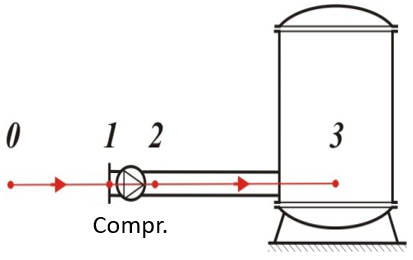
\includegraphics[scale=0.65]{figs/problem_1p5p9_compr_fig.png}
\caption{\label{gen_theprob}Compression system of Problem \thesection.\theprob.}
\end{center}
\end{figure}

\vspace{1cm}
\begin{tcolorbox}[breakable]
\noindent {\bf Problem \thesection.\theprob}\stepcounter{prob}

Find the input shaft work, the shaft power and the polytropic useful work of the previous problem! Calculate the pressure of the fluid in the tank after it cools down to the temperature of the
ambient fluid! Find the temperature assuming that the compression is an isentropic process! Neglecting the kinetic energy, find the useful work in case of an isentropic and isotherm process (the pressure
before and after the compressor can be assumed to be the same as for the politropic process).
\vspace{0.2cm}

Solution:
\vspace{0.2cm}

Calculate the input shaft work, the shaft power, and the polytropic useful work! The critical energy change of the air shall be considered.
\vspace{0.1cm}

$1$ – $2$: the compression can be approximated as a polytropic process.


Pressure of the air at the inlet: $p_1=p_0\left(\frac{T_1}{T_0}\right)^{\frac{\kappa}{\kappa-1}}=100 \cdot\left(\frac{279.3}{300}\right)^{\frac{1.4}{1.4-1}}=77.8 kPa$.
Density of the air at the inlet: $\rho_1=\frac{p_1}{RT_1}=279.3 \times \frac{77800}{286} \times 279.3=0.974 kg/m^3$.
The mass flow rate is: $\dot m=A_1\rho_1c_1=0.01227 \times 0.795 \times 203.7=2.436 kg/s$.


The temperature at the end of the compression is:
\begin{equation*}
	T_2=T_1\left(\frac{p_2}{p_1}\right)^{\frac{n-1}{n}}=279.3\left(\frac{4}{0.778}\right)^{\frac{1.54-1}{1.54}}.
\end{equation*}
The density of the air at the outlet of the compressor is: $\rho_2=\frac{p_2}{RT_2}=\frac{400000}{286 \times 495.5}=2.82 kg/m^3$.
The velocity of the air at the outlet of the compressor is: $c_2=\frac{\dot m}{A_2\rho_2}=\frac{2.436}{0.01227 \times 2.82}=70.4 m/s$.


The shaft work during the compression is:
\begin{equation*}
	Y_{in}=c_p(T_2-T_1)+\frac{{c_2}^2-{c_1}^2}{2}+g(z_2-z_1)=1001 \times (495.9-279.3)+\frac{{70.4}^2-{203.7}^2}{2}+0=199.9 kJ/kg.
\end{equation*}
The power of the compressor is:$P={\dot m}Y_{in}=2.436 \times 199.9=487 kW$.
The polytropic useful work is:
\begin{equation*}
	Y_{pol}=\frac{n}{n-1}\frac{p_1}{\rho_1}\left[\left(\frac{p_2}{p_1}\right)^{\frac{n-1}{n}}\right]=\frac{1.54}{1.54-1}\times\frac{77800}{0.974}\left[\left(\frac{4}{0.778}\right)^{\frac{1.54-1}{1.54}}\right]=176.7 kJ/kg.
\end{equation*}
As the air in the closed tank reaches its equilibrium state, is cools down to the ambient
temperature. Calculate the pressure in the tank after the air reaches the ambient temperature!
The cooling of the air in the tank (which is marked as number three in the figure) can be
approximated as an isochoric process (Gay-Lussac II. law, $p/T$ = const.)
\begin{equation*}
	p_3=p_2\frac{T_3}{T_2}=p_2\frac{T_0}{T_2}=400000 \times \frac{300}{495.7}=2.42 bar.
\end{equation*}
Calculate the useful work, if the compression process is assumed to be (i) isentropic or (ii)
isothermal. The pressure at the end of the compression should be the same as in the case of
the polytropic process!
Useful works: $p_1 -> p_2=4 bar$
Isentropic:
\begin{equation*}
	Y_{isentropic}=\frac{\kappa}{\kappa-1}\frac{p_1}{\rho_1}\left[\left(\frac{p_2}{p_1}\right)^{\frac{\kappa-1}{\kappa}}\right]=\frac{1.4}{1.4-1}\times\frac{77800}{0.974}\left[\left(\frac{4}{0.778}\right)^{\frac{1.4-1}{1.4}}\right]=166.8 kJ/kg.
\end{equation*}
Isothermal:
\begin{equation*}
	Y_{isothermal}=RT_1ln\left(\frac{p_2}{p_1}\right)=286 \times 279.3 \times ln\left(\frac{4}{0.778}\right)=130.8 kJ/kg
\end{equation*}
(which is the actual useful work, considering that the air cools down in the tank).
The shaft work is: $Y_in = 199,9 kJ/kg = 200 kJ/kg$. 
\end{tcolorbox}

\vspace{1cm}
\begin{tcolorbox}
\noindent {\bf Problem \thesection.\theprob}\stepcounter{prob}

Calculate the efficiency in the case of the different processes of the previous problem.
\vspace{0.2cm}

Solution:
\vspace{0.2cm}

From the value of the input/shaft work and
the useful work, the efficiency can be calculated in the case of the different processes.

\begin{equation*}
	\eta_{isothermal}=\frac{Y_{isothermal}}{Y_{in}}=\frac{130.8}{199.9}=0.654
\end{equation*}

\begin{equation*}
	\eta_{isentropic}=\frac{Y_{isentropic}}{Y_{in}}=\frac{166.8}{199.9}=0.834
\end{equation*}

\begin{equation*}
	\eta_{pol}=\frac{Y_{pol}}{Y_{in}}=\frac{176.4}{199.9}=0.882
\end{equation*}

In the figure below (Figure \ref{gen_fig}), the h-s diagram of dry air is displayed. The red curves are the isochore
($v=1/\rho=const.$) curves, while the black curves are the isobar ($p=const.$). The compression
process is displayed by the blue 0–1–2–3 lines.
\end{tcolorbox}
\vspace{1cm}

\begin{figure}[ht]
\begin{center}
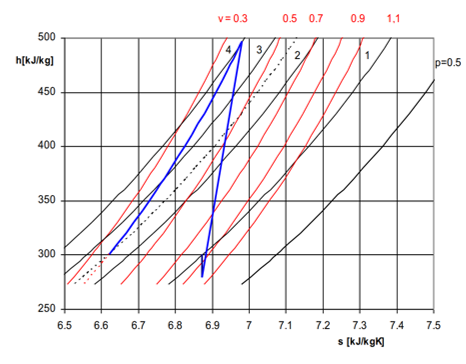
\includegraphics[scale=0.75]{figs/problem_1p5p11_fig.png}
\caption{\label{gen_fig}h-s diagram of dry air}
\end{center}
\end{figure}	

\vspace{0.7cm}
\noindent {\bf Problem \thesection.\theprob}\stepcounter{prob} 

At the pressure side of the compressor $2.5\,\mathrm{bar}$ absolute pressure and $187^{\circ}C$ temperature was measured,  the temperature of the inflow air is $27^{\circ}C$, and the pressure at the suction side is $1020\,\mathrm{hPa}$ ($1\,\mathrm{hPa}=100\,\mathrm{Pa}$). Find the politropic exponent of the compression and the politropic efficiency of the process, if $\kappa=1.4$! (Solution: $n=1.911$, $\eta_{pol}=0.6$).


\clearpage
